\chapter{Workshop introduction} 

Prescribed burning occupies a curious juncture between two stark realities in natural resource management: The rift between science and managers, and the complexity of fire as a natural phenomenon. 
Those said to \emph{know something about fire} rarely understand more than one or two facets of it, and struggle to communicate with other professionals across the scientist/manager divide. 

The concept of \emph{wildland fire science literacy} (Fig.~\ref{fig:WalletCard}) is rooted in the idea that  mutual understanding of three fundamental principles can facilitate effective communication\textemdash followed by collaborative thinking, action, and success\textemdash among scientists, managers, and even policy-makers:

\begin{quote}
	Wildland fire science literacy is the capacity for wildland fire professionals to understand and communicate three aspects of wildland fire: (1) the fundamentals of fuels and fire behavior, (2) the concept of fire as an ecological regime, and (3) multiple human dimensions of wildland fire and the socio-ecological elements of fire regimes \citep{mcgranahan2018}.
\end{quote}  

\begin{figure}
	\begin{center}
		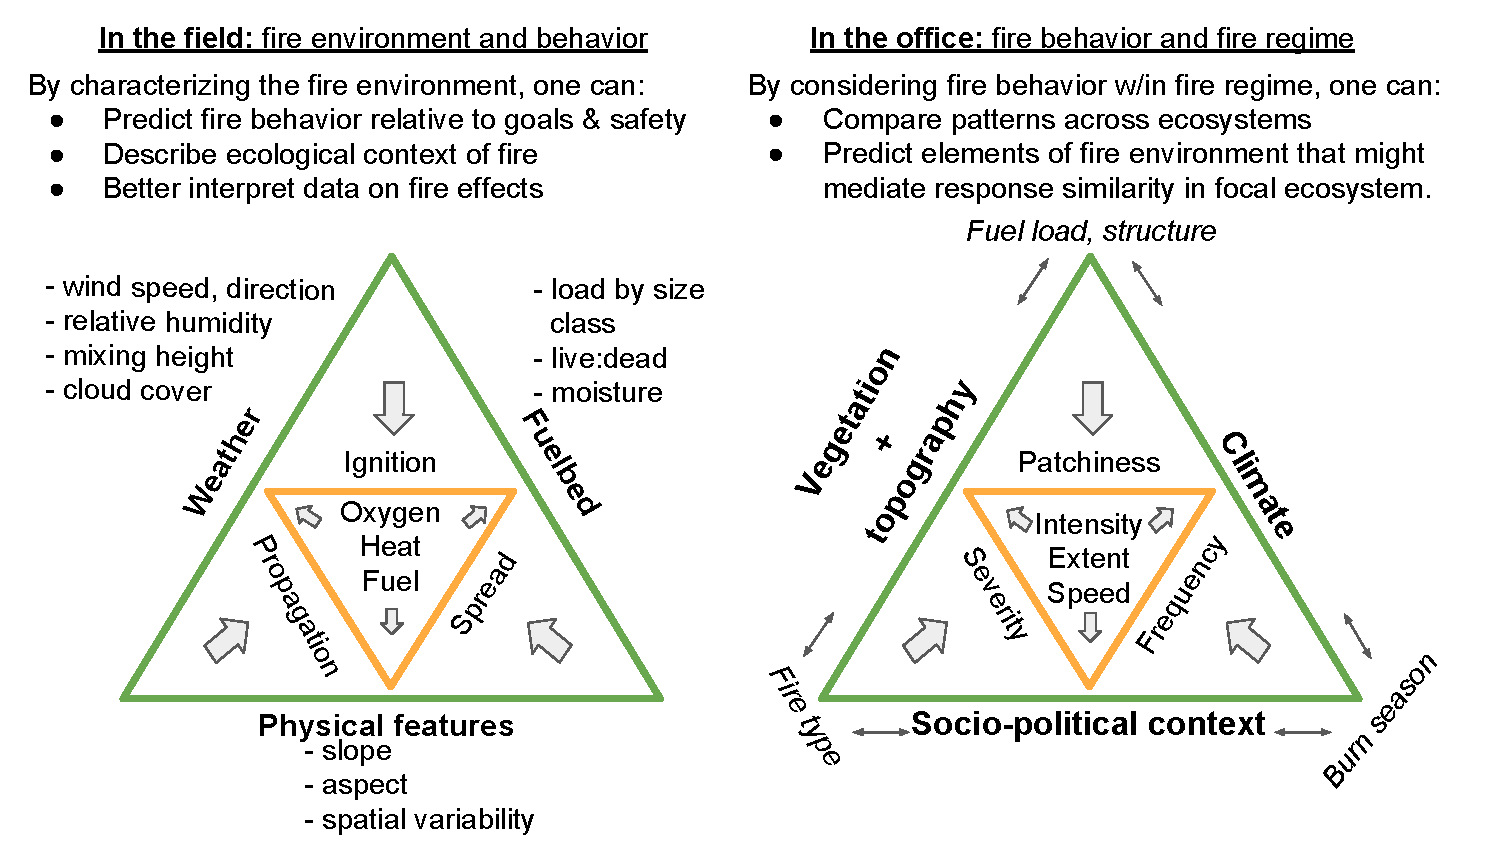
\includegraphics[width=1\textwidth]{WalletCard}
	\end{center}
	\caption{Two arenas of wildland fire science\textemdash the field and the office \citep{mcgranahan2018}. 
	This figure helps fire professionals from each arena identify characteristics of the fire environment or fire regime that dominate their colleagues' perspective.  
	\label{fig:WalletCard} }  %(Fig.~\ref{fig:WalletCard})
\end{figure}

This workshop has been designed to develop wildland fire science literacy by increasing the range of things fire professionals ``know something about'' when it comes to prescribed fire science and management. 
We hope that those who study prescribed fire have a better appreciation for what goes in to conducting an operation safely and effectively, and start to get some ideas on how to conduct better science in the management context.  
We hope that those who aim to use fire research have a more critical eye for what constitutes useful knowledge, in terms of both best practices in the science and transferability across management areas. 
And we hope that those who manage prescribed fire directly develop their critical thinking skills in assessing the \emph{what}, \emph{why}, and \emph{how} of burning as part of an ecological disturbance regime, and aim for more than just turning acres black. 

